% !TeX spellcheck = de_CH
\chapter{Bellsche Ungleichung\label{chapter:bell}}
\lhead{Bellsche Ungleichung}
\begin{refsection}
\chapterauthor{Hannes Badertscher}

In diesem Kapitel betrachten wir ein Gedankenexperiment von Albert Einstein
genauer.
Wie Randall Munroe von xkcd im Comic~\ref{fig:bell:xkcd_einstein} illustriert,
konnten die Theorien von Einstein bisher selten widerlegt werden.
Als einziges Beispiel, Einstein zu widerlegen, wird eine m\"oglicherweise
falsche Entscheidung Einsteins aufgef\"uhrt, als er bei seiner Arbeit im
Patentamt ein umstrittenes Patent zur Annahme empfahl.
Nat\"urlich entspricht dies nicht ganz der Wahrheit.
Wir uns in diesem Kapitel mit der Arbeit von Albert Einstein und versuchen
diese kritisch zu beleuchten.

\begin{figure}[b]
    \centering
    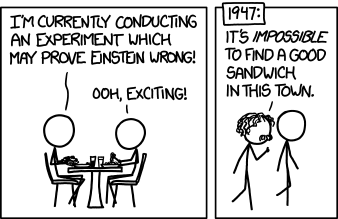
\includegraphics[width=0.5\linewidth]{bell/images/xkcd_einstein.png}
    \caption{XKCD Comic, welches darauf anspielt, dass sich kaum Fehler 
    in den Arbeiten von Albert Einstein finden lassen \cite{Bell:XkcdEinstein}}
    \label{fig:bell:xkcd_einstein}
\end{figure}

Im Mai 1935 ver\"offentlichten Albert Einstein, Boris Podolsky und
Nathan Rosen ein Gedankenexperiment mit welchem sie erkl\"arten, wieso
die Quantenmechanik nicht vollst\"andig sein kann. Als Alternative
sollten zus\"atzliche, verborgene Variablen eingef\"ugt werden, welche
das zugrunde liegende Verhalten logisch erkl\"aren k\"onnen.
W\"ahrend Niels Bohr die bisherige (Kopenhagen-) Interpretation der 
Quantenmechanik verteidigte, befassten sich diverse Physiker mit die Suche
nach solchen verborgenen Variablen.
In vielen Bereichen der Quantenmechanik wurden tats\"achlich
kleinere Teilchen, Quantenzahlen und Variablen entdeckt, welche das
Verst\"andnis der heutigen Quantenphysik pr\"agten.
Zur L\"osung des Gedankenexperiments von Einstein, Rosen und Podolsky konnten
jedoch bisher keine zus\"atzlichen Variablen gefunden werden.

Wir betrachten das Gedankenexperiment von Einstein, indem wir zuerst die
grundlegenden Annahmen der Lokalit\"at und des Realismus betrachten. Danach
gehen wir auf das von Einstein, Rosen und Podolski ver\"offentlichte Paradoxon
ein und kommen auf die darauf basierende Bellsche Ungleichung, welche
1961 von John Bell ver\"offentlicht wurde.

\section{Definitionen\label{section:bell:definitionen}}
Zuerst stellt sich die Frage der Anforderungen an die Theorie der
Quantenmechanik.
In diesem Abschnitt werden diese Anforderungen kurz definiert und
besprochen, sodass diesbez\"uglich keine Unklarheiten entstehen.
Albert Einstein stellte dabei die folgenden beiden Anforderungen an eine
Theorie:

\begin{enumerate}
    \item Lokalit\"at
    \item Realismus
\end{enumerate}

Die zentrale Eigenschaft ist die Lokalit\"at.
Diese besagt, dass jegliche Vorg\"ange nur einen Einfluss
auf ihre direkte Umgebung haben k\"onnen.

\begin{definition}\label{def:bell:lokalitaet}
    Eine physikalische Theorie ist \emph{lokal}, wenn zwei \"ortlich getrennte
    Systeme keinen sofortigen Einfluss aufeinander haben k\"onnen.
\end{definition}

\foreignquote{english}{Spooky actions at a distance} \cite[S.~158]{Bell:BornEinstein1971}
konnte sich Einstein nicht vorstellen.
Zum Beispiel war klassische Newtonsche Gravitationstheorie
eine \emph{nicht}-lokale Theorie. 
Eine Masse hat in der Gravitation sofort, ohne zeitliche 
Verz\"ogerung, einen Einfluss auf andere Massen -- unabh\"angig von der
r\"aumlichen Distanz zwischen den beiden Massen. 
In der speziellen Relativit\"atstheorie wurden die Begriffe von Raum und Zeit
so definiert, dass sich alle Materie und Energie h\"ochstens mit
Lichtgeschwindigkeit fortbewegen kann. 
Die allgemeine Relativit\"atstheorie ist eine alternative Formulierung
der Newtonschen Gravitationstheorie, welche die in der speziellen
Relativit\"atstheorie geforderte Lokalit\"at erf\"ullt.
Einstein war sich deshalb sicher, dass auf f\"ur die Quantenmechanik eine
Theorie herleiten l\"asst, in welcher sich jegliche Ereignisse h\"ochstens mit
Lichtgeschwindigkeit ausbreiten k\"onnen.

Mit der Forderung des Realismus wird verlangt, dass die Theorie eine
physikalische \emph{Realit\"at} beschreibt.
Das heisst dass eine Messung immer einen vorbestimmten Wert hat, und dieser
g\"ultig ist und existiert, ob die Messung durchgef\"uhrt wird oder nicht.

\begin{definition}\label{def:bell:}
    Eine physikalische Theorie ist \emph{realistisch}, wenn das Ergebnis
    jeglicher Messungen vorbestimmt ist.
\end{definition}

In einem Gespr\"ach mit Abraham Pais verdeutlichte Albert Einstein diese
Forderung mit dem bekannten Spruch
\foreignquote{english}{Do you really believe that the moon exists only when you look at it?}\cite{Bell:Pais1979}



\section{Das Einstein-Podolsky-Rosen Paradoxon\label{section:bell:epr}}
Das Einstein-Podolsky-Rosen Paradoxon (EPR Paradoxon) ist ein 
Gedankenexperiment, welches 1935 im Paper \cite{Bell:Einstein1935}
\enquote{Can quantum-mechanical description of physical reality be considered complete?}
von Albert Einstein, Boris Podolsky und Nathan Rosen publiziert wurde.
Einstein \emph{et al.} beginnen das Paper mit zwei Fragen zur
Quantenmechanik:

\begin{enumerate}
    \item Ist die Theorie korrekt?
    \item Ist die Beschreibung durch die Theorie vollst\"andig?
\end{enumerate}

Nur wenn beide diese Fragen mit \enquote{ja} beantwortet werden k\"onnen, 
ist die Theorie eine zufriedenstellende Beschreibung der Realit\"at.
Ob eine Theorie als korrekt bezeichnet werden kann wird definiert mit:

\begin{definition}\label{def:bell:Korrektheit}
    Die Korrektheit einer Theorie wird anhand des Grades der \"Ubereinstimmung
    zwischen den Vorhersagen einer Theorie und den entsprechenden praktischen
    Messungen und Experimenten.
\end{definition}

Diese Frage kann einfach gepr\"uft werden, indem die Resultate von
Experimenten mit den Vorhersagen der Theorie verglichen werden. 
Die Quantenmechanik konnte dabei, wie wir in diesem Buch in zahlreichen
Anwendungen nachvollziehen konnten, die Wirklichkeit korrekt vorhersagen. 
Um die zweite Frage zu diskutieren, definieren wir die Vollst\"andigkeit einer
Theorie wie folgt:

\begin{definition}\label{def:bell:Vollstaendigkeit}
    Jedes Element der physikalischen Realit\"at muss durch die Theorie
    genau beschrieben werden k\"onnen.
\end{definition}

Einstein, Podolsky und Rosen gehen in ihrem Paper genauer auf die Frage
der Vollst\"andigkeit der Quantenmechanik ein.
Dazu pr\"asentieren sie ein Gedankenexperiment, anhand welchem bewiesen
werden soll, dass die Quantenmechanik nicht vollst\"andig ist.
W\"ahrend Einstein \emph{et al.} das Gedankenexperiment sehr
allgemein hielten, diskutieren wir hier ein anschaulicheres Beispiel, welches
1957 von David Bohm und Yakir Aharonov \cite{Bell:Bohm1957} pr\"asentiert
wurde.

\subsection{Das Gedankenexperiment\label{subsection:bell:epr:idee}}
Wir betrachten zwei quantenmechanische Systeme, $I$ und $II$,
welche von $t=0$ bis zu einem Zeitpunkt $t=T$ miteinander 
interagieren k\"onnen. Darauf ist keine Interaktion mehr m\"oglich.
Visualisiert wird das Gedankenexperiment durch eine Quelle, welche
Elektron-Positron Paare emittiert. 
Dabei wird das Elektron (System $I$) zu einem Detektoren $A$ und das 
Positron (System $II$) zu einem Detektoren $B$ gesandt.
Diese sind physikalisch getrennt, sodass kein Informationsaustausch
zwischen den Detektoren m\"oglich ist.
Der Messaufbau ist in \figurename~\ref{fig:bell:EPR_Messaufbau} abgebildet.

\begin{figure}
    \centering
    \includegraphics{bell/images/experiment_setup.pdf}
    \caption{Messaufbau im Gedankenexperiment von EPR}
    \label{fig:bell:EPR_Messaufbau}
\end{figure}

Diese zwei Partikel werden so generiert, dass sie einen komplement\"aren
Spin-Zustand besitzen. 
Durch das Gesetz der Drehimpulserhaltung
ist dies einfach m\"oglich, da der Gesamtdrehimpuls eines Elektron-Positron 
Paares $+\frac12 - \frac12 = 0$ betr\"agt.

Wenn also bei Detektor $A$ der Spin des Elektrons entlang der $z$-Achse
gemessen wird und das Messresultat $+z$ ist, so ist sofort klar, dass
das das Positron bei Detektor $B$ den Spin $-z$ besitzen muss. 
Ebenso wird, falls bei Detektor $A$ der Spin entlang der $x$-Achse als $+x$
gemessen wird, das Positron bei Detektor $B$ den Spin $-x$ besitzen.

Wie im Kapitel der Heisenbergschen Unsch\"arferelation 
(Kapitel~\ref{chapter:heisenberg})
erkl\"art wird, sind die Messungen des Spins in verschiedenen Dimensionen 
komplement\"are Operatoren.
Damit ist es unm\"oglich, gleichzeitig beide Eigenschaften eines Teilchens
beliebig genau zu kennen.
Wird nun jedoch bei Detektor $A$ der Spin des Elektrons in $z$-Richtung 
als $+z$ gemessen, so ist bekannt dass das Positron den Spin $-z$ besitzt.
Da jedoch noch keine Messung am Positron ausgef\"uhrt wurde, kann bei
Detektor $B$ der Spin in $x$-Richtung gemessen werden.
Es ist also m\"oglich f\"ur das Positron gleichzeitig die exakten Werte 
des Spins in $x$-, wie in $z$-Richtung zu kennen. 
Mit der uns bekannten Beschreibung der Quantenmechanik mit Wellenfunktionen
kann dieser Effekt \emph{nicht} beschrieben werden, womit wir zu der
logischen Schlussfolgerung Einsteins kommen:

\begin{satz}
    Die quantenmechanische Beschreibung der physikalischen Realit\"at mittels
    Wellenfunktionen ist keine vollst\"andige Theorie.
\end{satz}

\subsection{Mathematische Herleitung\label{subsection:bell:epr:herleitung}}
Anhand des Spins kann das EPR Paradoxon einfach mathematisch formuliert werden.
Dabei wird die Notation aus Kapitel~\ref{chapter:spin} (\nameref{chapter:spin})
verwendet.

Wie in den Gleichungen~\ref{spin:paulimatrizen}--\ref{spin:vektoroperator}
hergeleitet wird der Spin-Operator durch die hermiteschen Pauli-Matrizen
beschrieben.

\begin{align}
    S_x &= \frac{\hbar}{2} \begin{pmatrix}
    0 & 1 \\ 1 & 0
    \end{pmatrix}
    &
    S_y &= \frac{\hbar}{2} \begin{pmatrix}
    0 & -i \\ i & 0
    \end{pmatrix}
    &
    S_z &= \frac{\hbar}{2} \begin{pmatrix}
    1 & 0 \\ 0 & -1
    \end{pmatrix}\label{equ:bell:paulimatrizen}
\end{align}

Wie in Abschnitt~\ref{subsection:bell:epr:idee} erkl\"art, betrachten wir
den Spin in $x$- und $z$-Richtung.
Die Eigenwerte der entsprechenden Pauli-Matrizen betragen:

\begin{align}
    |{+}x\rangle &= \frac{1}{\sqrt{2}}\begin{pmatrix} 1\\1 \end{pmatrix} &
    |{-}x\rangle &= \frac{1}{\sqrt{2}}\begin{pmatrix} 1\\-1 \end{pmatrix} &
    & \text{und} & 
    |{+}z\rangle &= \begin{pmatrix} 1\\0 \end{pmatrix} &
    |{-}z\rangle &= \begin{pmatrix} 0\\1 \end{pmatrix} &
\end{align}

Der Spin-Zustand $|\psi\rangle$ entlang der $z$-Achse eines 
Elektron-Positron Paares  kann durch alle m\"oglichen Kombination der beiden
Spins von Elektron und Positron beschrieben werden. 
Diese umfassen $+z$ f\"ur das Elektron und $-z$
f\"ur das Positron, sowie $-z$ f\"ur das Elektron und $+z$ f\"ur das Positron.
Zur Notation dieser kombinierten Zust\"ande wird das Tensorprodukt verwendet.

\begin{definition}\label{def:bell:tensorprodukt}
    Das Tensorprodukt von zwei Vektoren $A,B \in \mathbb{C}^2$  wird geschrieben als
    \[
        A \otimes B
    \]
    und entspricht der Abbildung $(\mathbb{C}^2,\mathbb{C}^2)\to\mathbb{C}^4$, 
    bei welcher jedes Element von $A$ mit jedem Element von $B$ multipliziert
    wird.
    Seien
    \begin{align*}
        A = \begin{pmatrix} a_{1} \\ a_{2} \end{pmatrix}
        &&
        B = \begin{pmatrix} b_{1} \\ b_{2} \end{pmatrix}
    \end{align*}
    so ist das Tensorprodukt
    \[
        A \otimes B = \begin{pmatrix} 
        a_1 b_1 & a_2 b_1 \\ a_1 b_2 & a_2 b_2
        \end{pmatrix}
    \]
\end{definition}

Damit ist der Zustand des Systems $|\psi\rangle$ definiert als

\begin{equation}
    |\psi\rangle = \frac{1}{\sqrt{2}} \Big( 
        |{+}z\rangle \otimes |{-}z\rangle - |{-}z\rangle \otimes |{+}z\rangle
     \Big)
     \label{equ:bell:spinstate}
\end{equation}

und somit

\begin{align}
    |\psi\rangle &= \frac{1}{\sqrt{2}} 
    \left( 
        \begin{pmatrix} 1\\0 \end{pmatrix} 
        \otimes 
        \begin{pmatrix} 0\\1 \end{pmatrix}
        -
        \begin{pmatrix} 0\\1 \end{pmatrix}
        \otimes
        \begin{pmatrix} 1\\0 \end{pmatrix}
     \right)
     =
     \frac{1}{\sqrt{2}}\left(
         \begin{pmatrix} 0 & 1 \\ 0 & 0 \end{pmatrix}
         -
         \begin{pmatrix} 0 & 0 \\ 1 & 0 \end{pmatrix}
     \right)
     \stackrel{!}{=}
     \frac{1}{\sqrt{2}}\left(
         \frac{1}{2}
         \begin{pmatrix} \phantom{-}1 & \phantom{-}1 \\ -1 & -1 \end{pmatrix}
         -
         \frac{1}{2}
         \begin{pmatrix} \phantom{-}1 & -1 \\ \phantom{-}1 & -1 \end{pmatrix}
     \right)  \notag \\
     &=
    -\frac{1}{\sqrt{2}} \left( 
        \frac{1}{\sqrt{2}}\begin{pmatrix} 1 \\ 1 \end{pmatrix} 
        \otimes 
        \frac{1}{\sqrt{2}}\begin{pmatrix} \phantom{-}1 \\ -1 \end{pmatrix}
        -
        \frac{1}{\sqrt{2}}\begin{pmatrix} \phantom{-}1 \\ -1 \end{pmatrix}
        \otimes
        \frac{1}{\sqrt{2}}\begin{pmatrix} 1 \\ 1 \end{pmatrix} 
     \right) \notag  \\
      &= 
      -\frac{1}{\sqrt{2}} \Big( 
              |{+}x\rangle \otimes |{-}x\rangle - |{-}x\rangle \otimes |{+}x\rangle
           \Big)\label{equ:bell:psix}
\end{align}

Wir haben also gezeigt, dass der Spin-Zustand $|\psi\rangle$ des
Elektron-Positron Paares \"aquivalent in Abh\"angigkeit des $z$-, sowie
des $x$-Spin Zustands geschrieben werden kann.
Wird nun bei Detektor $A$ der Spin des Elektrons in $z$-Richtung gemessen, 
so findet eine Projektion des Zustands $|\psi\rangle$ auf entweder
$|{+}z\rangle$ oder $|{-}z\rangle$ statt.
Der Zustand reduziert sich auf
\begin{align*}
    |\psi_{1}\rangle &= |{+}z\rangle \otimes |{-}z\rangle
    & \text{bzw.} && 
    |\psi_{2}\rangle &= |{-}z\rangle \otimes |{+}z\rangle
\end{align*}
Damit ist der Spin in $z$-Richtung f\"ur das Positron bei Detektor $B$ ohne
eine Messung vorbestimmt, n\"amlich als $-z$ im ersten Fall bzw. $+z$ im
zweiten Fall.
Wenn nun bei Detektor $B$ der Spin des Positrons in $x$-Richtung gemessen
wird, so wird der urspr\"ungliche Spin-Zustand $|\psi\rangle$
ebenfalls reduziert auf
\begin{align*}
    |\psi_{a}\rangle &= |{+}x\rangle \otimes |{-}x\rangle
    & \text{bzw.} && 
    |\psi_{b}\rangle &= |{-}x\rangle \otimes |{+}x\rangle
\end{align*}
Wir erhalten damit zwei Wellenfunktionen, z.B. $|\psi_{1}\rangle$ und 
$|\psi_{a}\rangle$, welche \emph{gleichzeitig} die gleiche 
physikalische Realit\"at beschreiben.
Um zu pr\"ufen ob dies im Fall des Spin-Zustands \"uberhaupt m\"oglich 
ist, wenden wir Hilfssatz~\ref{skript:kommutatorannihliertev} an.
Der Kommutator $[S_x,S_z]$ ist
\begin{equation}
    [S_x, S_z] =  -i \hbar S_y \neq 0
\end{equation}
Da die Operatoren $S_x$ und $S_z$ also nicht vertauschen, ist nach der Theorie
der Quantenmechanik die gleichzeitige Kenntnis der beiden Messungen \emph{nicht}
m\"oglich.
Dass dies jedoch hier der Fall ist, haben wir in Abschnitt~\ref{subsection:bell:epr:idee}
hergeleitet und mathematisch in diesem Abschnitt beweisen k\"onnen.
Damit m\"ussen wir zur Schlussfolgerung kommen, dass entweder 
(1) eine sofortige Kommunikation zwischen dem Elektron und dem Positron
stattfindet, was  jedoch durch die Lokalit\"at ausgeschlossen wird,
oder (2) dass die Beschreibung der Quantenmechanik mittels der Wellenfunktion
nicht  vollst\"andig ist und ein fundamentaler, nicht messbarer, Mechanismus
bestimmt welches Ergebnis eine Messung des Spins ergeben wird.


\subsection{Die Theorie der verborgenen lokalen Variablen}
Besinnen wir uns zur\"uck auf die beiden initialen Fragen: 
(1) \enquote{Ist die Theorie korrekt?} und 
(2) \enquote{Ist die Beschreibung durch die Theorie vollst\"andig?}
Dabei mussten wir feststellen, dass zwar die Frage (1) dank diverser
Experimente mit \enquote{ja} beantwortet werden kann, doch die Frage (2) 
durch das besprochene Gedankenexperiment nur mit \enquote{nein} beantwortet
werden kann. 
Damit stellt sich die Frage, um welches Element die Theorie der Quantenmechanik
erweitert werden muss, sodass die Beschreibung vollst\"andig wird.

Eine m\"ogliche L\"osung des Paradoxons wurde bereits in
Abschnitt~\ref{subsection:bell:epr:herleitung} kurz beschrieben:
Es k\"onnte ein verborgener Mechanismus existieren, welcher das Resultat unseres
Experiments, also den Spin von Elektron und Positron, vorausbestimmt.
Dazu wird eine verborgene Variable eingef\"uhrt, welche das
Resultat der Spin-Messung bestimmt. 
Diese wird als \emph{verborgene} Variable bezeichnet, da sie nicht
messbar ist, sondern nur die Auswirkungen der Variable, also der jeweilige
Spin, gemessen werden kann.
Um das durch Einstein, Rosen und Podolski eingef\"uhrte Paradoxon zu l\"osen
reicht eine 2-dimensionale Variable $\lambda\in\mathbb{C}^2$ aus, 
welche den Zusammenhang zwischen dem Spin in $x$- und $z$-Richtung beschreibt.

Eine Visualisierung der m\"oglichen Werte von $\lambda$ ist in 
Abbildung~\ref{fig:bell:hidden_var} dargestellt.
Liegt die Variable $\lambda$ im ersten Quadranten des Diagramms, so ist 
unabh\"angig von der Messung $A$ eindeutig bestimmt, dass der Spin des Elektrons
sowohl in $x$-, wie in $z$-Richtung positiv sein wird.
Damit ist auch klar, dass der Spin des Positrons in $x$- und in $z$-Richtung
negativ sein wird.

\begin{figure}
    \centering
    \includegraphics{bell/images/hidden_vars.pdf}
    \caption{Visualisierung der verborgenen Variable $\lambda$ des Spin-Zustands}
    \label{fig:bell:hidden_var}
\end{figure}

Die Variable $\lambda$ ist lokal, da sie in der Quelle auf einen Wert gesetzt
wird, und alle m\"oglichen Spin-Messungen an den beiden Teilchen von da an
definitiv bestimmt sind.
Sie ist verborgen, da $\lambda$ nicht direkt messbar ist, sondern nur
anhand von zwei Spin-Messungen bei den Detektoren $A$ und $B$ bestimmt werden 
kann.
Mit dieser Theorie lassen sich die beiden Forderungen Einsteins, die Lokalit\"at
und der Realismus, erf\"ullen und die um verborgene lokale Variablen erweiterte
Quantenmechanik w\"are vollst\"andig.
Die Herausforderung eine solche Variable $\lambda$ wirklich 
in Form eines existierenden Teilchens zu finden bleibt jedoch bestehen.

\section{Die Bellsche Ungleichung\label{section:bell:bell}}
Nach der Ver\"offentlichung des EPR Paradoxons gingen verschiedene bekannte
Physiker auf das Paradoxon ein.
Niels Bohr, Mitbegr\"under der Kopenhagen Interpretation der Quantenmechanik,
antwortete bereits 1935 mit einer eher schwammigen Widerlegung Einsteins
\cite{Bell:Bohr1935}.
Bohr ging dabei gar nicht auf die Unvollst\"andigkeit der Quantenmechanik ein,
sondern argumentierte dass die Quantenmechanik konsistent sein muss -- was
Einstein zu diesem Zeitpunkt gar nicht infrage stellte.
Im Nachhinein betrachtet musste 1949 sogar Bohr selbst zugeben, dass seine
Reaktionen auf Einstein \enquote{ineffizient} waren und 
\enquote{es schwierig machten darauf zu antworten}. 

Erwin Schr\"odinger hingegen zweifelte nicht am EPR Paradoxon selbst, sondern
\"ausserte Zweifel daran, dass diese Beschreibung f\"ur \"ortlich getrennte
quantenmechanische Systeme ebenfalls gilt und damit ob der Effekt auch
messbar ist \cite{Bell:Schroedinger1936}.

David Bohm entwickelte in \cite{Bell:Bohm1952} eine Theorie auf Basis
lokaler verborgener Variablen in Anlehnung an Einsteins Gedankenexperiment.
Dabei betrachtete er nicht  Position und Drehmoment, wie im Paper von EPR,
sondern den Spin zweier Partikel.
Dieses Gedankenexperiment ist einfacher zu analysieren (weshalb wir im
Abschnitt~\ref{section:bell:epr} das Experiment von Bohm, und nicht das
originale von Einstein betrachtet haben).

Als sich John Bell, noch als Student, mit dem EPR Paradoxon und insbesondere
der Arbeit von David Bohm zu besch\"aftigen begann, kamen ihm insbesondere
Zweifel an der Lokalit\"at dieser verborgenen Variablen.
In seinem ber\"uhmten Paper
\enquote{On the Einstein Podolsky Rosen Paradox} \cite{Bell:Bell1964}
gelang es ihm zu beweisen, dass eine Theorie der verborgenen Variablen -- sollte
eine solche existieren -- \emph{nicht} lokal sein kann.
Als erstem Physiker gelang es die Frage umzudrehen, und nicht nach solchen
Variablen bzw. Teilchen zu suchen, sondern gleich deren Nicht-Existenz
zu beweisen.

Wir betrachten das Paper von Bell indem wir uns erneut das Gedankenexperiment 
nach Abbildung~\ref{fig:bell:EPR_Messaufbau} befassen.
Dazu verallgemeinern wir das Experiment etwas und betrachten zuerst die
Vorhersage mittels der Quantenmechanik.
Da diese ja korrekt, aber noch nicht vollst\"andig ist, f\"uhren wir darauf
eine lokale, verborgene Variable $\lambda$ ein und berechnen deren Vorhersage.
Auf Basis dieser beider Resultate leiten wir die Bellsche Ungleichung, und
darauf eine verallgemeinerte Version, die BCHSH-Ungleichung her.

\subsection{Vorhersage der Quantenmechanik}
Der Spin eines Teilchens in einer beliebigen Richtung $\vec{a}$, wobei $\vec{a}$
ein Einheitsvektor ist, wird durch die
Projektion der Spin-Matrix des Teilchens $A$ auf die 
Richtung $\vec{a}$ gemessen.
\begin{equation}\label{equ:bell:meas_a}
    \vec{\hat{\sigma}}_A \cdot \vec{a}
\end{equation}
Dies kann mithilfe der Pauli-Matrizen \eqref{equ:bell:paulimatrizen} geschrieben
werden als
\begin{align}
    \vec{a} \cdot \vec{\hat{\sigma}}_A &= 
    a_1 \hat{\sigma}_x + a_2 \hat{\sigma}_y + a_3 \hat{\sigma}_z = 
    a_1 \begin{pmatrix} 0 & 1 \\ 1 & 0 \end{pmatrix} +
    a_2 \begin{pmatrix} 0 & -i \\ i & 0 \end{pmatrix} + 
    a_3 \begin{pmatrix} 1 & 0 \\ 0 & -1 \end{pmatrix} \\
    & = \begin{pmatrix}
       a_3 & a_1 - i a_2 \\
       a_1 - i a_2 & -a_3
    \end{pmatrix} \label{equ:bell:proj_a_s}
\end{align}
Der Spin-Zustand $|\psi\rangle$ des Elektron-Positron Paares kann mit
\eqref{equ:bell:meas_a} und $\vec{\hat{\sigma}}_B \cdot \vec{b}$ 
f\"ur das Teilchen $B$ als Superposition der beiden
Spin-Zust\"ande bei $A$ und $B$ geschrieben werden:
\begin{equation}
    |\psi\rangle = \left( \vec{\hat{\sigma}}_A \cdot \vec{a} \right)
        \otimes \left( \vec{\hat{\sigma}}_B \cdot \vec{b} \right)
\end{equation}
Der Erwartungswert $E_{QM}$ des Produkts der zwei Spin-Messungen
ist daher
\begin{equation}\
    E_{QM} = \left\langle \phi \left| 
    \left( \vec{\hat{\sigma}}_A \cdot \vec{a} \right)
            \otimes \left( \vec{\hat{\sigma}}_B \cdot \vec{b} \right)
    \right| \phi \right\rangle
\end{equation}
Da die Messung jeweils entweder $|+\rangle$ oder $|-\rangle$ ergibt, kann
dies analog zu \eqref{equ:bell:spinstate} umgeformt werden.
\begin{equation} 
\begin{split}
   E_{QM }=&\left\langle \phi \left| 
       \left( \vec{\hat{\sigma}}_A \cdot \vec{a} \right)
               \otimes \left( \vec{\hat{\sigma}}_B \cdot \vec{b} \right)
       \right| \phi \right\rangle
    = \\
    \frac{1}{2}\Bigg[ &
        \left\langle{+}\left| \vec{\hat{\sigma}}_A \cdot \vec{a} \right|{+}\right\rangle_A
        \left\langle{-}\left| \vec{\hat{\sigma}}_B \cdot \vec{b} \right|{-}\right\rangle_B
        -
        \left\langle{+}\left| \vec{\hat{\sigma}}_A \cdot \vec{a} \right|{-}\right\rangle_A
        \left\langle{-}\left| \vec{\hat{\sigma}}_B \cdot \vec{b} \right|{+}\right\rangle_B \\
        - &
        \left\langle{-}\left| \vec{\hat{\sigma}}_A \cdot \vec{a} \right|{+}\right\rangle_A
        \left\langle{+}\left| \vec{\hat{\sigma}}_B \cdot \vec{b} \right|{-}\right\rangle_B
        +
        \left\langle{-}\left| \vec{\hat{\sigma}}_A \cdot \vec{a} \right|{-}\right\rangle_A
        \left\langle{+}\left| \vec{\hat{\sigma}}_B \cdot \vec{b} \right|{+}\right\rangle_B
    \Bigg]
\end{split}
\end{equation}
Was mit \eqref{equ:bell:proj_a_s} vereinfacht werden kann zu
\begin{equation}\label{equ:bell:e_qm}
\begin{split}
    E_{QM} &= \frac{1}{2} \big[ -a_3b_3 - (a_1-ia_2)(b_1+ib_2) - (a_1+ia_2)(b_1-ib_2) - a_3b_3 \big] \\
    &= -\big[ a_1b_1 + a_2b_2 + a_3b_3 \big] \stackrel{!}{=} -\vec{a} \cdot \vec{b}
\end{split}
\end{equation}
Da $\vec{a}$ und $\vec{b}$ Einheitsvektoren sind, gilt
\begin{equation}
    \vec{a} \cdot \vec{b} = \cos(\theta_{ab}) \qquad \text{f\"ur} \quad |\vec{a}| = |\vec{b}| = 1
\end{equation}
mit dem Winkel $\theta_{ab}$ zwischen $\vec{a}$ und $\vec{b}$.
Somit wird der quantenmechanische Erwartungswert zu
\begin{equation}\label{equ:bell:res_qm}
    E_{QM}(\vec{a},\vec{b}) = -\vec{a}\cdot\vec{b} = -\cos(\theta_{ab})
\end{equation}

\subsection{Vorhersage mittels verborgener Variablen}
Nehmen wir nun an, dass eine Theorie der verborgenen Variablen vorliegt
und eine Variable $\lambda \in \Lambda$ existiert.
\"Uber die Art dieser Variable, ob kontinuierlich oder diskret, wird hier keine
Annahme gemacht.
Die Wahrscheinlichkeitsverteilung dieser Variable sei $\rho(\lambda)$, womit gilt
\begin{equation}\label{equ:bell:lambdaverteilung}
    \int_{\lambda\in\Lambda} \rho(\lambda) d\lambda = 1
\end{equation}
Damit diese Theorie die Quantenmechanik erweitern kann, muss sie die Vorhersage
der Quantenmechanik mit dem Erwartungswert 
$E_{QM}(\vec{a},\vec{b}) = -\vec{a}\cdot\vec{b}$
ebenfalls f\"ur alle Richtungen $\vec{a}$ und $\vec{b}$ produzieren.
Die Messungen $A(\vec{a})$ und $B(\vec{b})$ h\"angen nun also von einer
vorbestimmten Variable $\lambda$ ab.
\begin{equation}\label{equ:bell:messungen_ab}
    A(\vec{a}) \cdot B(\vec{b})(\lambda) = A(\vec{a},\lambda) \cdot B(\vec{b},\lambda)
\end{equation}
mit
\begin{equation}\label{equ:bell:werte_ab}
    A(\vec{a},\lambda) = \pm 1 \qquad \text{und} \qquad B(\vec{b},\lambda) = \pm 1
\end{equation}
Aus \eqref{equ:bell:lambdaverteilung} und \eqref{equ:bell:messungen_ab}
l\"asst sich der Erwartungswert des Produkts der beiden Spin-Messungen
bestimmen als
\begin{equation}\label{equ:bell:e_lambda}
    E(\vec{a},\vec{b}) = \int_{\lambda\in\Lambda} 
        \rho(\lambda) A(\vec{a},\lambda) B(\vec{b},\lambda) d\lambda
\end{equation}
Aufgrund des Messaufbaus und \eqref{equ:bell:res_qm} gilt f\"ur 
$\vec{a} = \vec{b}$:
\[
    -1 = \int_{\lambda\in\Lambda} 
        \rho(\lambda) A(\vec{a},\lambda) B(\vec{a},\lambda) d\lambda
\]
Diese perfekte Antikorrelation ist nur bei
\begin{equation}\label{equ:bell:antikorrelation}
    A(\vec{a},\lambda) = -B(\vec{a},\lambda)
\end{equation}
erf\"ullt.
Damit wird \eqref{equ:bell:e_lambda} zu
\begin{equation}\label{equ:bell:e_lambda_vereinf}
    E(\vec{a},\vec{b}) = -\int_{\lambda\in\Lambda} 
        \rho(\lambda) A(\vec{a},\lambda) A(\vec{b},\lambda) d\lambda
\end{equation}

\subsection{Herleitung der Bellschen Ungleichung}
Aus dieser vereinfachten Gleichung l\"asst sich nun die Bellsche Ungleichung
herleiten.
Dazu wird neben den beiden Richtungen $\vec{a}$ und $\vec{b}$ eine dritte,
unabh\"angige Richtung $\vec{c}$ betrachtet. 
$\vec{c}$ ist ebenfalls ein Einheitsvektor.
Aufgrund von \eqref{equ:bell:werte_ab} gilt, dass
$|A(\vec{b},\lambda)|^2 = 1$ ist.
Wir betrachten nun die Differenz zweier Erwartungswerte
$E(\vec{a},\vec{b}) - E(\vec{a},\vec{c})$:
\begin{equation}\label{equ:bell:diff_e}
\begin{split}
    E(\vec{a},\vec{b}) - E(\vec{a},\vec{c}) =
    - \int_{\lambda\in\Lambda} \rho(\lambda) \left[ 
        A(\vec{a},\lambda) A(\vec{b},\lambda) - 
        A(\vec{a},\lambda) A(\vec{c},\lambda)
    \right] d\lambda \\
    = \int_{\lambda\in\Lambda} \rho(\lambda)A(\vec{a},\lambda)A(\vec{b},\lambda)
        \left[ A(\vec{b},\lambda)A(\vec{c},\lambda) - 1 \right] d\lambda
\end{split}
\end{equation}
Um die Bellsche Ungleichung herleiten zu k\"onnen, wird 
Hilfssatz~\ref{hilfssatz:bell:dreiecksungleichung_integral}
eingef\"uhrt.
\begin{hilfssatz}\label{hilfssatz:bell:dreiecksungleichung_integral}
    Sei $Z$ eine auf dem Intervall $\Omega$ integrierbare Funktion, so gilt
    \[
        \left|\int_{\Omega} Z\, d\mu\,\right| 
        \leq \int_{\Omega} |\,Z\,|\, d\mu
    \]
\end{hilfssatz}
\begin{proof}
    Beweis nach \cite{Bell:HilfssatzTriangle}.
    Es wird $\alpha\in\mathbb{C}$ mit $|\alpha| = 1$ gew\"ahlt, sodass
    \[
        \alpha \cdot \int_{\Omega} Z\, d\mu = 
        \left|\int_{\Omega} Z\, d\mu\,\right|
    \]
    Damit ist
    \[
        \left|\int_{\Omega} Z\, d\mu\,\right| = 
        \operatorname{Re}\left( \int_{\Omega}\alpha Z \,d\mu \right) = 
        \int_{\Omega}\operatorname{Re}(\alpha Z)\,d\mu
        \leq
        \int_{\Omega} |\,\alpha Z\,|\, d\mu = 
        \int_{\Omega} |\,Z\,|\, d\mu
    \]
\end{proof}

Die Differenz \eqref{equ:bell:diff_e} wird nun mithilfe von
Hilfssatz~\ref{hilfssatz:bell:dreiecksungleichung_integral} geschrieben als
\begin{equation}
\begin{split}
    |E(\vec{a},\vec{b}) - E(\vec{a},\vec{c})| =
    \left| \int_{\lambda\in\Lambda} \rho(\lambda)
        A(\vec{a},\lambda)A(\vec{b},\lambda)
        \left[ A(\vec{b},\lambda)A(\vec{c},\lambda) - 1 \right]
        d\lambda
    \right| \\
    \leq 
    \int_{\lambda\in\Lambda} \left|  
        \rho(\lambda)A(\vec{A},\lambda)A(\vec{b},\lambda)
        \left[ A(\vec{b},\lambda)A(\vec{c},\lambda) - 1 \right]
    \right| d\lambda
\end{split}
\end{equation}
Der Term auf der rechten Seite wird nun mithilfe von $|A(\cdot,\lambda)|=1$
weiter vereinfacht zu
\begin{align*}
    &= \int_{\lambda\in\Lambda} \rho(\lambda) \left|
    A(\vec{a},\lambda)A(\vec{c},\lambda) - A(\vec{a},\lambda)A(\vec{b},\lambda)
    \right| d\lambda \\
    &= \int_{\lambda\in\Lambda} \rho(\lambda)
    \left| A(\vec{a},\lambda) \right| \cdot 
    \left| A(\vec{c},\lambda) - A(\vec{b},\lambda) \right| d\lambda \\
    &= \int_{\lambda\in\Lambda} \rho(\lambda)
    \left|\left[ A(\vec{b},\lambda) A(\vec{c},\lambda) - 1 \right]\right| d\lambda \\
    &= \int_{\lambda\in\Lambda} \rho(\lambda) 
    \left[1 - A(\vec{b},\lambda)A(\vec{c},\lambda) \right] d\lambda \\
    &= \int_{\lambda\in\Lambda} \rho(\lambda) d\lambda
    - \int_{\lambda\in\Lambda} \rho(\lambda) 
    (\vec{b},\lambda)A(\vec{c},\lambda) d\lambda
\end{align*}
Damit sind wir wieder bei einem Erwartungswert der Form von
\eqref{equ:bell:e_lambda_vereinf} und k\"onnen die erste Form der Bellschen
Ungleichung \cite[(15)]{Bell:Bell1964} aufstellen:
\begin{equation}\label{equ:bell:bellsche_ungleichung}
    \left| E(\vec{a},\vec{b}) - E(\vec{a},\vec{c}) \right| 
    \leq
    1 + E(\vec{b},\vec{c})
\end{equation}

Diese Ungleichung muss, wenn eine Theorie lokaler, verborgener Variablen 
vorliegt, f\"ur alle Richtungen $\vec{a}$, $\vec{b}$ und $\vec{c}$ gelten.
Betrachten wir als Beispiel die Messrichtungen
\begin{align*}
    \vec{a}\cdot\vec{b} = \frac{\pi}{4} &&
    \vec{b}\cdot\vec{c} = \frac{\pi}{4} &&
    \vec{a}\cdot\vec{c} = 0
\end{align*}
welche in Abbildung~\ref{fig:bell:orientierung_pi4} dargestellt sind.
Werden die Erwartungswerte der Quantenmechanik nach 
\eqref{equ:bell:e_lambda_vereinf} berechnet und in die Bellsche Ungleichung
eingesetzt, folgt

\begin{figure}
    \centering
    \includegraphics{bell/images/orientierung_pi4.pdf}
    \caption{Visualisierung der Messrichtungen, welche eine Verletzung der
    Bellschen Ungleichung durch die Quantenmechanik ergeben.}
    \label{fig:bell:orientierung_pi4}
\end{figure}

\[
    \frac{1}{\sqrt{2}} \nleqslant 1 - \frac{1}{\sqrt{2}}
\]

Mit den gew\"ahlten Orientierungen ergibt sich also ein Widerspruch. 
Die Quantenmechanik verletzt die Bellsche Ungleichung, welche f\"ur jede Theorie
mit lokalen verborgenen Variablen gelten muss.
Daraus kann geschlossen werden, dass das EPR Gedankenexperiment von keiner
Theorie lokaler verborgener Variablen erkl\"art werden kann, und sich Albert
Einstein damit get\"auscht hat.

Die Bellsche Ungleichung \eqref{equ:bell:bellsche_ungleichung} l\"asst sich
experimentell jedoch nur schwer \"uberpr\"ufen, da unter anderem in
\eqref{equ:bell:antikorrelation} eine perfekte Antikorrelation der Messungen
gefordert wird, was in der Praxis nur schwer realisiert werden kann.

\subsection{Herleitung der CHSH Ungleichung}
Um reale experimentelle Bedingungen nachbilden zu k\"onnen, passten
John Clauser, Michael Horne, Abner Shimony und Richard Holt 
\cite{Bell:Clauser1969} die Bellsche Ungleichung so an, dass die perfekte
Korrelation nicht notwendig ist.
Ihr Resultat wird als CHSH-Ungleichung bezeichnet, war aber ebenfalls noch nicht
f\"ur reale Experimente geeignet.
Erst John Bell, der sich von den Fortschritten von Clauser \textit{et al.}
anspornen liess und nach 7 Jahren sich wieder mit dem Thema besch\"aftigte,
konnte eine pr\"ufbare Version der Bellschen Ungleichung herleiten, die so
genannte \enquote{Bell-Clauser-Horne-Shimony-Holt (BCHSH) Ungleichung}. 

Dabei wird ber\"ucksichtigt, dass die Korrelation nicht perfekt ist, sondern
um ein $\delta$ von $-1$ abweichen kann:
\begin{equation}
    E(\vec{a},\vec{b}) = -1 + \delta 
    \qquad \text{mit} \quad  0 \leq \delta \leq 1     
    \qquad \text{f\"ur} \quad |\vec{a}| = |\vec{b}| = 1
\end{equation}
Weiter wird \eqref{equ:bell:werte_ab} so erweitert, dass die Nicht-Detektion
eines Teilchens m\"oglich ist:
\begin{equation}
    A(\vec{a},\lambda) = \begin{cases}
        +1 & \text{Spin Up} \\
        -1 & \text{Spin Down} \\
        0 & \text{nicht detektiert}
    \end{cases}
\end{equation}
Als weiteres Zugest\"andnis an reale Messbedingungen werden nicht mehr einzelne
Messungen $A(\vec{a},\lambda)$ betrachtet, sondern mehrere Messungen zu
$\bar{A}(\vec{a},\lambda)$ gemittelt.
Damit wird \eqref{equ:bell:werte_ab} zu
\begin{equation}
    \left| \bar{A}(\vec{a},\lambda) \right| \leq 1
    \qquad \text{und} \qquad 
    \left| \bar{B}(\vec{b},\lambda) \right| \leq 1
\end{equation}

Nun werden statt die 3 Messrichtungen $\vec{a}$, $\vec{b}$ und $\vec{c}$
insgesamt 4 Richtungen eingef\"uhrt: $\vec{a}, \vec{a'}, \vec{b}, \vec{b'}$
und die Differenz $E(\vec{a},\vec{b}) - E(\vec{a},\vec{b}')$ betrachtet:
\begin{equation}
    E(\vec{a},\vec{b}) - E(\vec{a},\vec{b}') = 
    \int_{\lambda\in\Lambda} \rho(\lambda) \left[
        \bar{A}(\vec{a},\lambda)\bar{B}(\vec{b},\lambda) -
        \bar{A}(\vec{a},\lambda)\bar{B}(\vec{b'},\lambda)
    \right] d\lambda
\end{equation}
Diese wird analog zur Herleitung der Bellschen Ungleichung 
\eqref{equ:bell:bellsche_ungleichung} umgeformt und vereinfacht, und wir
erhalten schlussendlich
\[
    \left| E(\vec{a},\vec{b}) - E(\vec{a},\vec{b}') \right| \leq \pm \left[
        E(\vec{a}',\vec{b}') + E(\vec{a}',\vec{b})
    \right]
    + 2 \int_{\lambda\in\Lambda} \rho(\lambda) d\lambda
\]
was wir mit einem letzten Schritt zur BCHSH-Ungleichung umformen k\"onnen
\begin{equation}\label{equ:bell:bchsh-ungleichung}
    -2 \leq 
    E(\vec{a},\vec{b}) - E(\vec{a},\vec{b'}) + E(\vec{a'},\vec{b}) + E(\vec{a'},\vec{b'})
    \leq 2
\end{equation}
Betrachten wir nun die in Abbildung~\ref{fig:bell:orientierung_2}
abgebildeten Messrichtungen
\begin{align*}
    \vec{a}\cdot\vec{b} = \frac{\pi}{4} && 
    \vec{b}\cdot\vec{a}' = \frac{\pi}{4} && 
    \vec{a}'\cdot\vec{b}' = \frac{\pi}{4} 
\end{align*}
\begin{figure}
    \centering
    \includegraphics{bell/images/orientierung_2.pdf}
    \caption{Visualisierung der Messrichtungen, welche eine Verletzung der
    BCHSH Ungleichung durch die Quantenmechanik ergeben.}
    \label{fig:bell:orientierung_2}
\end{figure}
Das Einsetzen der Werte ergibt
\[
    2 \sqrt{2} \nleqslant 2
\]
womit die Quantenmechanik die BCHSH Ungleichung ebenfalls verletzt.

\section{Experimente}
Zur experimentellen \"Uberpr\"ufung der Bellschen Ungleichung werden meist
nicht, wie hier besprochen, Elektron-Positron-Paare verwendet, sondern
Photonen mit identischer Polarisation.
Dabei k\"onnen die Photon entweder vertikal ($+$) oder horizontal
($-$) polarisiert sein. 
Es ergibt sich der folgende Polarisationszustand:
\begin{equation}\label{equ:bell:photonstate}
    |\psi\rangle = \frac{1}{\sqrt{2}} \Big(
        |{+}\rangle \otimes |{+}\rangle + |{-}\rangle \otimes |{-}\rangle
    \Big)
\end{equation}
Wird nun die Polarisation der beiden Elektronen in der gleichen Richtung 
gemessen, sind die Messergebnisse perfekt korreliert.
Bei Richtungen mit einem Winkel von \SI{45}{\degree} wird das Resultat
unkorreliert sein, also komplett zuf\"allig.
Wird in einem Winkel von \SI{90}{\degree} gemessen, sind die Messergebnisse
anti-korreliert.

Die Erwartungswerte werden nun gesch\"atzt indem gez\"ahlt
wird, wie h\"aufig die m\"oglichen Resultat $++$, $+-$, $-+$ und $--$
vorkommen ($N_{++}, N_{+-}, N_{-+}, N_{--}$).
Der Erwartungswert $E_(\vec{a},\vec{b})$ einer Detektor-Einstellung 
$(\vec{a},\vec{b})$ wird nun berechnet durch
\begin{equation}
    E = \frac{N_{++} + N_{--} - N_{+-} - N_{-+}}{N_{++} + N_{--} + N_{+-} + N_{-+}}
\end{equation}
Die Bellsche Ungleichung wird \"uberpr\"uft, indem die vier Einstellungen
$(\vec{a},\vec{b})$, $(\vec{a},\vec{b}')$, $(\vec{a}',\vec{b})$
und $(\vec{a}',\vec{b}')$ gemessen und deren Erwartungswerte berechnet werden. 
Diese Werte werden in die Bellsche Ungleichung eingesetzt:
\begin{equation}
    S = E(\vec{a},\vec{b}) - E(\vec{a},\vec{b'}) + E(\vec{a'},\vec{b}) + E(\vec{a'},\vec{b'})
\end{equation}
Wenn das gemessene $S$ die Ungleichung \eqref{equ:bell:bchsh-ungleichung} 
$-2 \leq S \leq +2$
verletzt, so st\"utzt das Experiment die Ergebnisse der Quantenmechanik.
Kann nicht mit ausreichender statistischer Signifikanz belegt werden, dass
die Bellsche Ungleichung verletzt wird, so kann die Existenz verborgener
lokaler Variablen nicht ausgeschlossen werden.

\subsection{M\"ogliche Probleme}
Es gibt zahlreiche Herausforderungen bei der Entwicklung und der Durchf\"uhrung
solcher Experimente.
Die wichtigsten Probleme sind

\paragraph{Effizienz der Detektoren}
Die Entwicklung eines Detektoren, welcher einzelne Photonen detektieren muss,
gestaltet sich nicht als einfach, und die optimale Effizienz von $\eta = 1$ wird
nicht erreicht.
Je h\"oher die Effizienz der verwendeten Detektoren ist, desto gr\"osser ist die
Konfidenz in das Resultat der Messung. 

\paragraph{Sicherstellen der Lokalit\"at}
Im Experiment muss sichergestellt sein, dass die beiden Teilchen keine
keine Informationen \"uber die Messung austauschen k\"onnen.
Dazu m\"ussen die Detektoren so r\"aumlich getrennt werden, dass
der gesamte Messprozess bei beiden Detektoren beendet ist, bevor Informationen,
welche sich mit Lichtgeschwindigkeit ausbreiten, beim anderen Teilchen
ankommen k\"onnen. 

\paragraph{R\"aumliche Korrelation}
Neben der Anforderung, dass ein Photonenpaar mit gleicher Polarisation erzeugt
werden muss, m\"ussen die Photonen ebenfalls r\"aumlich so korreliert sein,
dass diese wirklich zum Detektor gelangen.
Dazu m\"ussen Betrag und Richtung des Impulses beider Photonen stark korreliert
sein. Dies wird in Abbildung~\ref{fig:bell:raum_korr} illustriert.

\begin{figure}
    \centering
    \includegraphics{bell/images/raum_korr.pdf}
    \caption{Sind die Photonen r\"aumlich nur schwach korreliert,
    so k\"onnen nicht notwendigerweise beide detektiert werden.}
    \label{fig:bell:raum_korr}
\end{figure}

\subsection{1. Generation -- Freedman Clauser (1972)}
Das erste Experiment, welches die Bellsche Ungleichung \"uberpr\"ufte,
wurde 1972 von Stuart Freedman und John Clauser an der UC~Berkeley
in Kalifornien durchgef\"uhrt \cite{Bell:Freedman1972}.
Dazu wurden Calcium-40 Atome in den Zustand $\text{3d}\,\text{4p}\,^1\text{P}_1$
angeregt. 
Wie in Abbildung~\ref{fig:bell:freedman} dargestellt wird ein Teil der
angeregten Atome direkt in den Grundzustand $\text{4s}^2\,^1\text{S}_0$
\"ubergehen, w\"ahrend etwa \SI{7}{\percent} der Atome \"uber die Kaskade
via $\text{4p}^2\,^1\text{S}_0$ und $\text{4p}\,\text{4s}\,^1\text{P}_1$ 
in den Grundzustand \"ubergehen.
Dabei werden zwei Photonen mit einer Wellenl\"ange von \SI{551.3}{\nano\meter}
bzw. \SI{442.7}{\nano\meter} freigesetzt. 
Da der Drehimpuls des Calcium Atoms $J=0$ betr\"agt, m\"ussen die Photonen
eine entgegengesetzte Polarisation haben.

\begin{figure}
    \centering
    \includegraphics{bell/images/freedman.pdf}
    \caption{Atomare Kaskade im Calcium Atom, welche zwei Photonen mit
    gegens\"atzlicher Polarisation erzeugt. \cite{Bell:Freedman1972}}
    \label{fig:bell:freedman}
\end{figure}

Mit diesem Experiment konnten Freedman und Clauser erstmals die Bellsche
Ungleichung testen und konnte eine klare Verletzung der Bellschen Ungleichung
messen.
Aufgrund einer sehr tiefen Detektor-Effizienz und nur schwacher r\"aumlicher
Korrelation der Photonen konnte jedoch, trotz Best\"atigung in mehreren 
\"ahnlichen Experimenten, die Existenz verborgener lokaler Variablen nicht
mit Sicherheit ausgeschlossen werden.

\subsection{2. Generation -- Alain Aspect (1980--1985)}
Anfang der 1980er Jahre wurde an der Universit\'e Paris-Sud in Orsay von Alain
Aspect im Rahmen seiner Dissertation eine Serie neuer Experimente zur Pr\"ufung
der Bellschen Ungleichung entwickelt und durchgef\"uhrt
\cite{Bell:Aspect1981,Bell:Aspect1982:1,Bell:Aspect1982:2}. 
Aspect verwendete dazu dieselbe atomare Kaskade wie Freedman Clauser, jedoch
wurden die Calcium Atome anders angeregt. 
Das Problem der Lokalit\"at wurde mittels eines optischen Schalters, welcher 
innerhalb von \SI{10}{\nano\second} zwischen den zu messenden 
Polarisationsrichtungen umschalten konnte, behandelt.
Damit wurde erst w\"ahrend die Photonen bereits auf dem Weg zum Detektor waren
definiert, welche Messung stattfinden soll.
Durch eine r\"aumliche Trennung von \SI{13}{\meter} zwischen den Detektoren
sollte dieses Problem also behandelt werden. 

Obwohl Aspect in allen Experimenten die Verletzung der Bellschen Ungleichung
best\"atigen konnte, blieben durch die weiterhin geringe Detektor-Effizienz,
sowie die geringe Distanz zwischen Detektoren Zweifel, ob die Bellsche
Ungleichung damit tats\"achlich best\"atigt werden kann.

\subsection{3. Generation}
Die Experimente der dritten Generation basieren auf einem neuen Verfahren
zur Erzeugung von Photonenpaaren, der parametrischen Fluoreszenz.
Dabei wird mittels eines Pumpstrahls mit Frequenz $\omega_p$ ein
nichtlinearer optischer Kristall angeregt.
Es entstehen durch den Satz der Energieerhaltung und $E_{ph}=\hbar \omega$
zwei Photonen mit Frequenzen $\omega_1$ und $\omega_2$, sodass 
$\omega_1 + \omega_2 = \omega_p$.
Damit lassen sich zwei Photonen mit derselben Polarisation erzeugen.
Mithilfe der Methode der parametrischer Fluoreszenz werden r\"aumlich
stark korrelierte Photonen erzeugt, was ein deutlicher Vorteil
gegen\"uber der Methode mit atomaren Kaskaden darstellt.
Dank der Einkopplung der Photonen in Glasfaserkabel konnten diverse neue
Experimente entwickelt werden.

\paragraph{Weihs, Innsbruck 1998}
Das Problem der Lokalit\"at konnte zum ersten Mal 1998 von einem Team
um Gregor Weihs in Innsbruck gel\"ost werden \cite{Bell:Weihs1998}.
Die Detektoren wurden dabei \SI{400}{\meter} voneinander getrennt platziert.
Damit bleibt eine Zeit von
\[
    t_c = \frac{s}{c} = \frac{\SI{400}{\meter}}{\SI{2.998e8}{\meter\per\second}} \approx \SI{1.3}{\micro\second}
\]
zur Messung.
Weihs entwickelte einen elektro-optischen Modulator, welcher die 
Polarisationsrichtung eines Photons um \SI{45}{\degree} drehen konnte und
mittels eines Zufallsgenerators gesteuert wurde.
Damit konnte sichergestellt werden, dass die Messrichtung wirklich zuf\"allig
ist.
Die gesamte Verz\"ogerung im Messsystem betrug etwa 
$t_m = \SI{100}{\nano\second}$, also deutlich unter $t_c = \SI{1.3}{\micro\second}$. 
Damit war das Team um Weihs das erste, welches das Problem der Lokalit\"at
beheben konnte.
Ihr Ergebnis,
\[
    S(\SI{0}{\degree},\SI{45}{\degree},\SI{22.5}{\degree},\SI{67.5}{\degree})
    = 2.73 \pm 0.02 \nleqslant 2
\]
konnte die Existenz einer Theorie der lokalen verborgenen Variablen klar 
ausschliessen.
Die Detektoreffizienz lag bei Weihs jedoch immer noch bei etwa \SI{5}{\percent},
womit nicht alle Zweifel am Resultat des Experiment behoben werden konnten.

\paragraph{Rowe, Boulder 2001}
Das erste Experiment, in welchem die Detektoreffizienz gen\"ugend hoch war um
alle Teilchen korrekt erkennen zu k\"onnen, wurde von Rowe \textit{et al.}
in Boulder, Colordo durchgef\"uhrt \cite{Bell:Rowe2001}. 
Durch die Verwendung von Beryllium-Ionen anstatt von Photonen konnte die
Detektoreffizienz auf \"uber \SI{90}{\percent} erh\"oht werden.
Auch Rowe kam in seinem Experiment mit
\[
    S(\SI{-22.5}{\degree},\SI{67.5}{\degree},\SI{-22.5}{\degree},\SI{67.5}{\degree})
    = 2.25 \pm 0.03 \nleqslant 2
\]
auf eine klare Verletzung der Bellschen Ungleichung.
Da die Beryllium-Ionen im Experiment jedoch nur \SI{3}{\micro\meter}
auseinander platziert werden konnten, wurden bereits behobene Probleme in
diesem Experiment wieder eingef\"uhrt.

\paragraph{Aktuelle Forschung}
Noch in keinem Experiment konnten gleichzeitig alle Probleme behandelt werden.
Obwohl der Einfluss aller beschriebener Effekte jeweils einzeln experimentell
ausgeschlossen werden konnte, kann noch nicht mit Sicherheit nachgewiesen
werden, dass die Bellsche Ungleichung durch die Quantenmechanik verletzt wird.
Die Existenz einer Theorie lokaler verborgener Variablen kann also noch nicht
ausgeschlossen werden. 
Aktuell wird daran geforscht, alle diese Probleme mit einem einzigen Experiment
beheben zu k\"onnen. 
Marissa Giustina (Wien, 2013) \cite{Bell:Giustina2013} konnte mit demselben 
Aufbau jegliche Zweifel ausr\"aumen -- jedoch nicht gleichzeitig, sondern in 
mehreren Messungen.
Es wird erwartet, dass in den n\"achsten Jahren ein Experiment durchgef\"uhrt
werden kann, welche jegliche Zweifel beseitigt und endg\"ultig nachweisen
kann, dass die Intuition von Einstein falsch war und keine verborgenen
lokalen Variablen existieren k\"onnen.

\section{Fazit}
In diesem Kapitel haben wir das Gedankenexperiment Einsteins genauer betrachtet
und feststellen m\"ussen, dass Einstein mit seiner Intuition zur Quantenmechanik
falsch lag.
Obwohl noch kein Experiment alle Zweifel beseitigen konnte, m\"usste man fast
an eine 
\enquote{Verschw\"orung der Natur} (A.~J.~Leggett, \cite{Bell:Leggett2003})
glauben um die Bellsche Ungleichung noch infrage zu stellen.

Der Traum Einsteins, eine physikalische Beschreibung der Realit\"at, welche sich
sowohl an die Lokalit\"at, wie auch an den Realismus h\"alt, kann somit nicht 
erf\"ullt werden.
Es existieren nun zwei m\"ogliche Auswege aus dieser Situation:
\begin{enumerate}[label=(\roman*)]
    \item Die Welt ist nicht-lokal. Damit wird das grundlegende Prinzip der
        Relativit\"at in Frage gestellt.
    \item Es existiert keine objektive Realit\"at. Damit k\"onnen wir keine
        gesicherten Aussagen \"uber weit entfernte Ereignisse machen.
\end{enumerate}
Welche dieser Annahmen das geringere \"Ubel ist, l\"asst sich nicht
abschliessend beurteilen -- fest steht nur, dass die Quantenmechanik
nicht lokal \emph{und} realistisch sein kann.

\printbibliography[heading=subbibliography]
\end{refsection}

